\documentclass{ctexart}
\usepackage{graphicx}

\begin{document}

\section{Introduction}

\subsection{Overall Objective}
本实验是EEE109电子电路课程的第2次实验，主题为BJT与放大器。实验通过NI ELVIS III平台，结合2N3904晶体管、测量仪器和仿真工具，分为五个部分进行：观测晶体管IV特性、分析晶体管开关行为、研究共射放大器的增益与频率响应、验证射极跟随器输出特性，以及完成一个综合电路设计任务。实验旨在巩固晶体管偏置和放大原理，培养理论分析与实验测量的结合能力。

\subsection{Theoretical Background}
NPN型双极结晶体管由基极、发射极和集电极组成。在有源区，基极-发射极结被正向偏置，集电极-基极结被反向偏置，此时集电极电流近似由基极电流控制，并由电流放大倍数$\beta$体现。晶体管的工作状态可分为截止区、饱和区和有源区：截止区时几乎没有集电极电流，饱和区时集电极-发射极压降很低，有源区则可实现线性放大。

共射放大电路依赖适当的偏置网络来建立稳定工作点，耦合电容和旁路电容则影响低频响应。放大器的电压增益由晶体管参数和负载电阻决定，输出通常与输入反相。射极跟随器的特点是输出电压几乎随输入变化，仅低于输入一个基极-发射极压降，因此具有高输入阻抗、低输出阻抗和近似单位电压增益，适用于阻抗匹配与信号缓冲。

\subsection{Expected Behaviour of the Circuits}
在第1部分中，随着集电极电压增加，BJT的集电极电流应在有源区趋于平稳，不同基极电流下的输出曲线应呈现出刻度式的分布，反映出$\beta$的变化。在第2部分中，晶体管作为开关时应显示出截断和饱和两种明显状态：截断时集电极电流近乎为零，饱和时$V_{CE}$显著降低。在第3部分中，共射放大器应给出反相输出，在中频范围内表现出稳定的电压增益，而在低频端由于耦合或旁路电容的影响会出现增益下降。在第4部分中，射极跟随器应实现输出紧随输入、幅度接近1且输出阻抗较低的特性。在第5部分的设计任务中，预期通过合理选择偏置和元件，得到符合规格的直流工作点和交流响应良好的电路。

\subsection{The Organization of the Report}
本报告首先以Abstract开头，总结实验目的、方法、结果和结论。随后Introduction部分介绍实验背景、目的、理论背景、电路预期行为以及报告组织。Experimental Setup and Procedures节描述实验设置、仪器和测量步骤。Results and Analysis节通过表格和图表展示并分析结果，与理论比较并讨论误差。最后Conclusion节总结实验确认的内容、意义和可靠性，References节列出引用资料。

\section{Experimental Setup and Procedures}

\subsection{Instruments and Components}
本实验采用NI ELVIS III硬件平台作为主要测量仪器。该平台集成了多种功能，包括可变电源、数字万用表（DMM）、IV分析仪、示波器等。实验所需的主要元器件包括：2N3904 NPN晶体管、各种阻值的电阻（如33~$\mathrm{k\Omega}$、100~$\mathrm{k\Omega}$、1~$\mathrm{k\Omega}$、8.2~$\mathrm{k\Omega}$、18~$\mathrm{k\Omega}$等）、电容（1~$\mu$F、100~$\mu$F）、1~$\mathrm{k\Omega}$和10~$\mathrm{k\Omega}$的可变电位器、1N4001和1N4735齐纳二极管。所有元器件均安装在NI ELVIS III配套的原型板（protoboard）上进行测试。

\subsection{Section 1: Bipolar Junction Transistor Characteristics}

\begin{center}
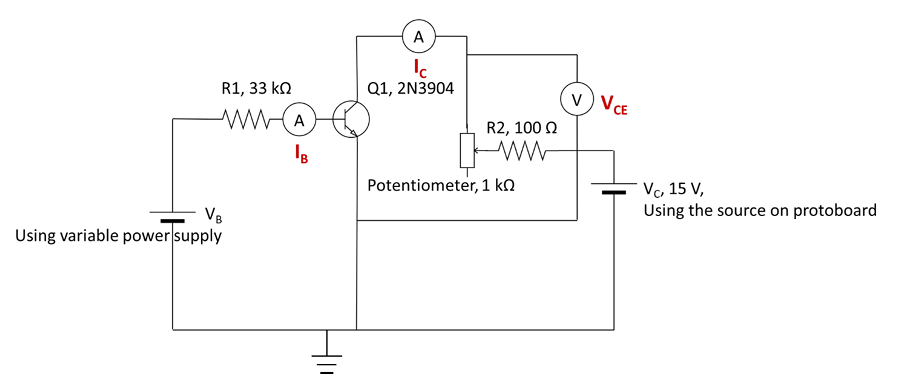
\includegraphics[width=0.50\textwidth]{Section1_Circuit_Diagram.png}

图：BJT特性测量电路原理图
\end{center}

在本部分中，首先使用NI ELVIS III的IV分析仪直接测量2N3904晶体管的输入输出特性。将晶体管的基极、集电极、发射极分别连接到IV分析仪的对应接口。设置分析仪参数：晶体管类型为NPN，集电极电压扫描范围0-3 V，基极电流从15 $\mu$A开始以11 $\mu$A步长增加，共5条曲线。系统自动生成IV特性曲线图。

之后，利用NI ELVIS III的可变电源和数字万用表手动测量BJT在有源区的工作特性。搭建测量电路如图Figure 1-2所示，通过调节可变电位器改变基极电流，分别设定基极电压为2.38 V、4.08 V、5.76 V三个工作点，在每个点上逐步改变集电极供电电压，记录对应的集电极-发射极电压和集电极电流。该方法能够验证晶体管在不同偏置条件下的电流放大系数$\beta$是否恒定。

在电路搭建过程中发现，该电路需要同时由面包板电源和函数发生器供电，并且多个接地点须统一接地。初期各接地点独立连接时，数字万用表的测量读数没有明显变化。将面包板的地线、电路接地点和函数发生器的地线统一连接后，电压表恢复正常工作。这充分说明在多电源协同工作的电路中，建立可靠的公共接地平面是保证测量精度和数据可靠性的关键。

\begin{center}
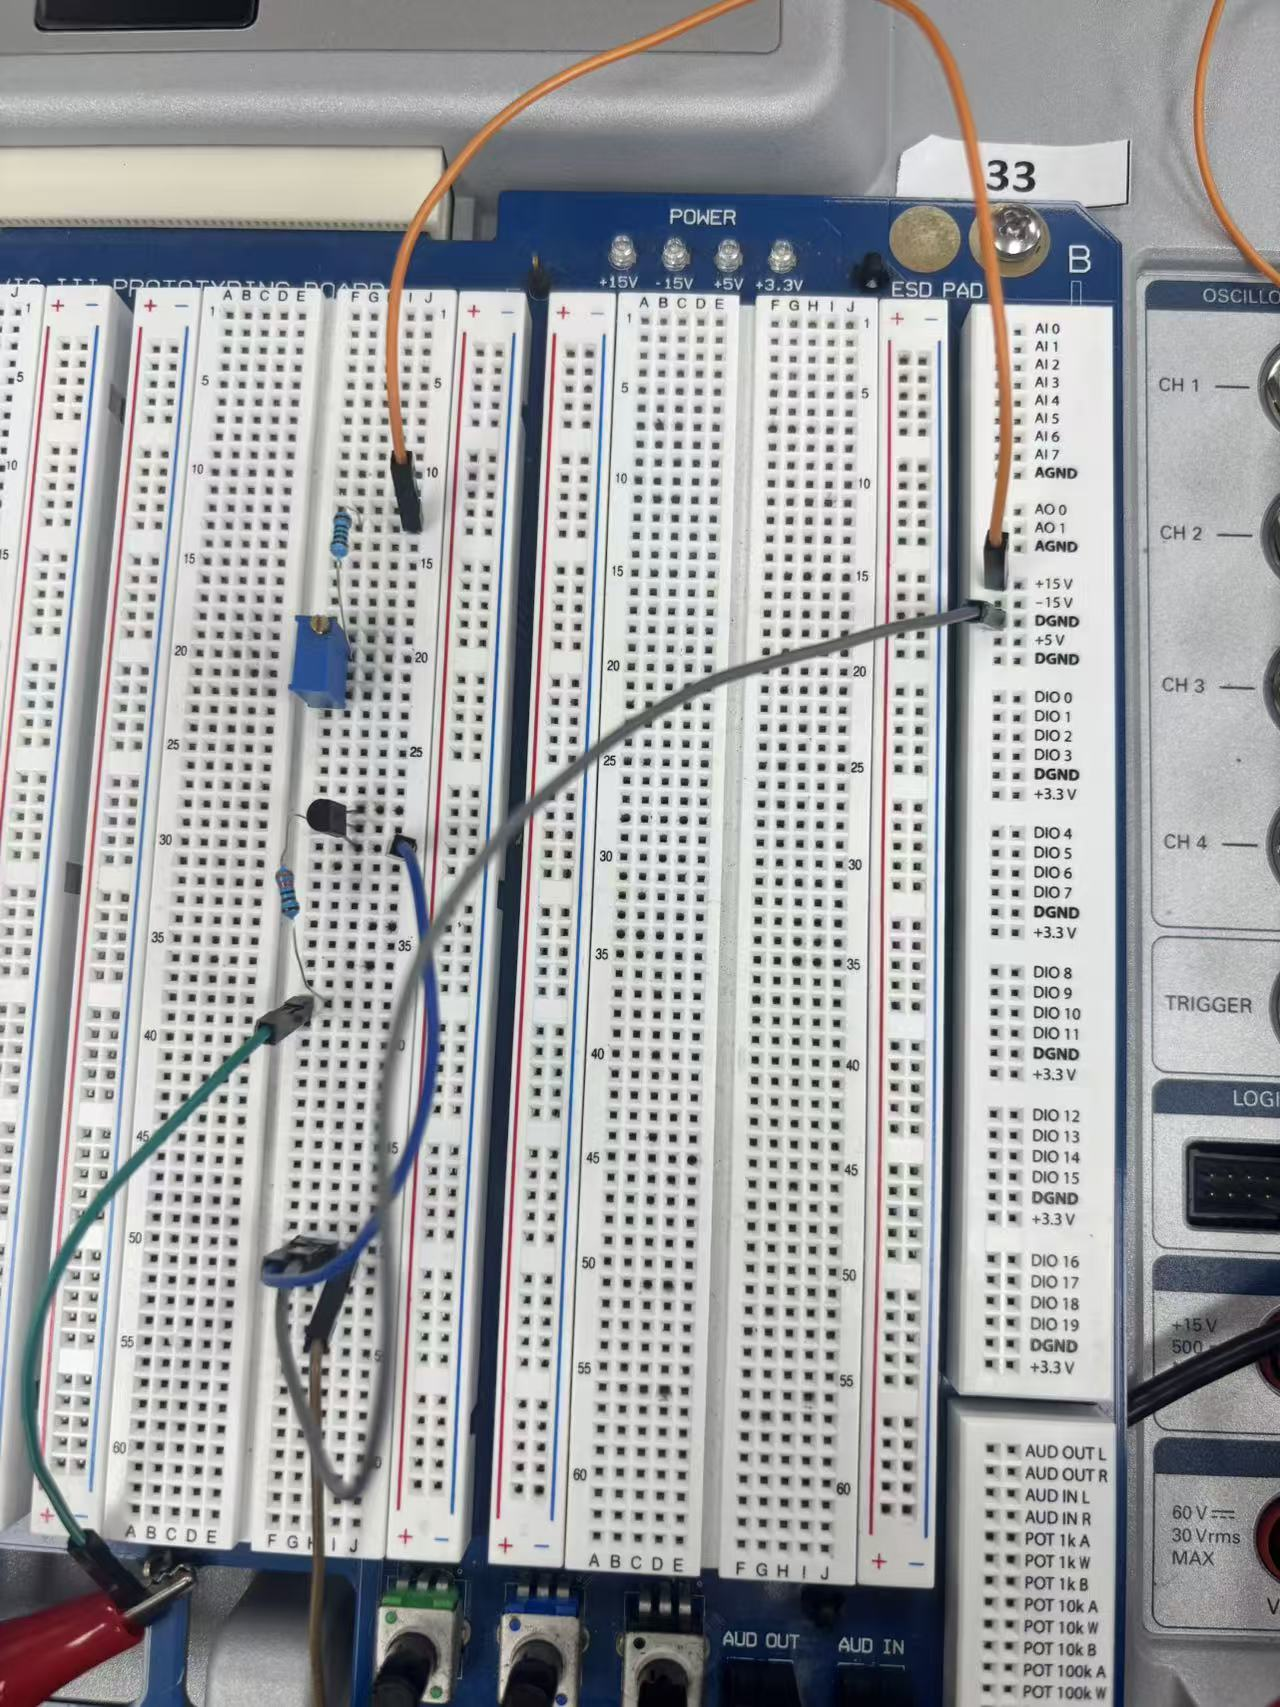
\includegraphics[width=0.50\textwidth]{Section1_BJT_Characteristics.jpg}

图：Section 1 晶体管特性测量电路实际搭建
\end{center}

\subsection{Section 2: BJT as a Switch}

\begin{center}
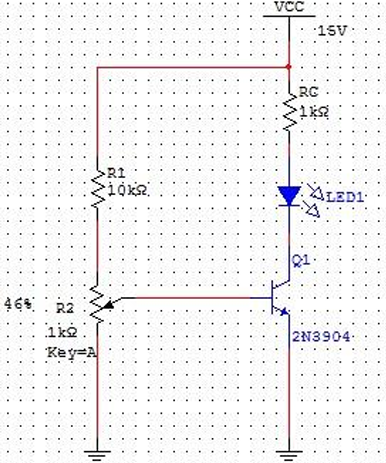
\includegraphics[width=0.45\textwidth]{Section2_Circuit_Diagram.png}

图：晶体管开关电路原理图
\end{center}

本部分主要通过理论计算分析晶体管作为开关时的行为。根据给定的负载电阻和供电电压，计算使晶体管完全饱和和完全截止所需的基极电流。分析表明，当基极电流足够大时（通常为负载电流的1/10以上），晶体管进入饱和区，此时集电极-发射极电压极低（约0.1-0.3 V）；反之，当基极电流为零时，晶体管截止，集电极电流接近零。该部分主要涉及计算，无需实际搭建电路。

\subsection{Section 3: Common Emitter Amplifier}

\begin{center}
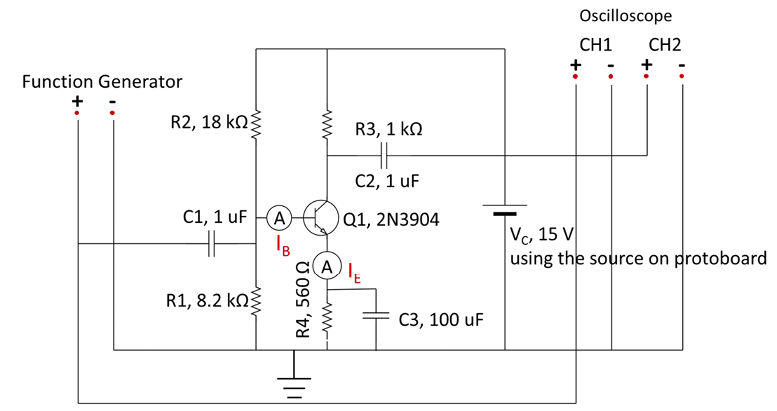
\includegraphics[width=0.50\textwidth]{Section3_Circuit_Diagram.png}

图：共射放大器电路原理图
\end{center}

本部分搭建一个共射放大电路，按照实验脚本的电路设计选择合适的偏置电阻和耦合电容。电路的偏置电阻设定工作点在有源区中点附近，耦合电容（1 $\mu$F）用于隔离直流分量，旁路电容（100 $\mu$F）用于增大交流增益。

使用NI ELVIS III的可变电源和DMM分别测量电路的直流工作点（基极、集电极、发射极电压）。然后通过信号发生器输入不同频率的正弦波信号（如1 kHz中频信号），用示波器或DMM测量输入和输出信号的幅度，计算电压增益。逐步扫描频率（如从100 Hz到100 kHz），绘制频率响应曲线，观察耦合和旁路电容对增益的影响。

在电路搭建和测试过程中，发现过度使用杜邦线会导致接触不良问题，进而严重影响信号质量和测量的可靠性。因此在电路搭建时应尽量减少杜邦线的使用，优先采用直接连接法。此外，需要特别注意防止电阻和电容的引脚相互接触或与其他部分短接，这些细节虽然看似微小，但对实验的成功和数据的有效性至关重要。

\begin{center}
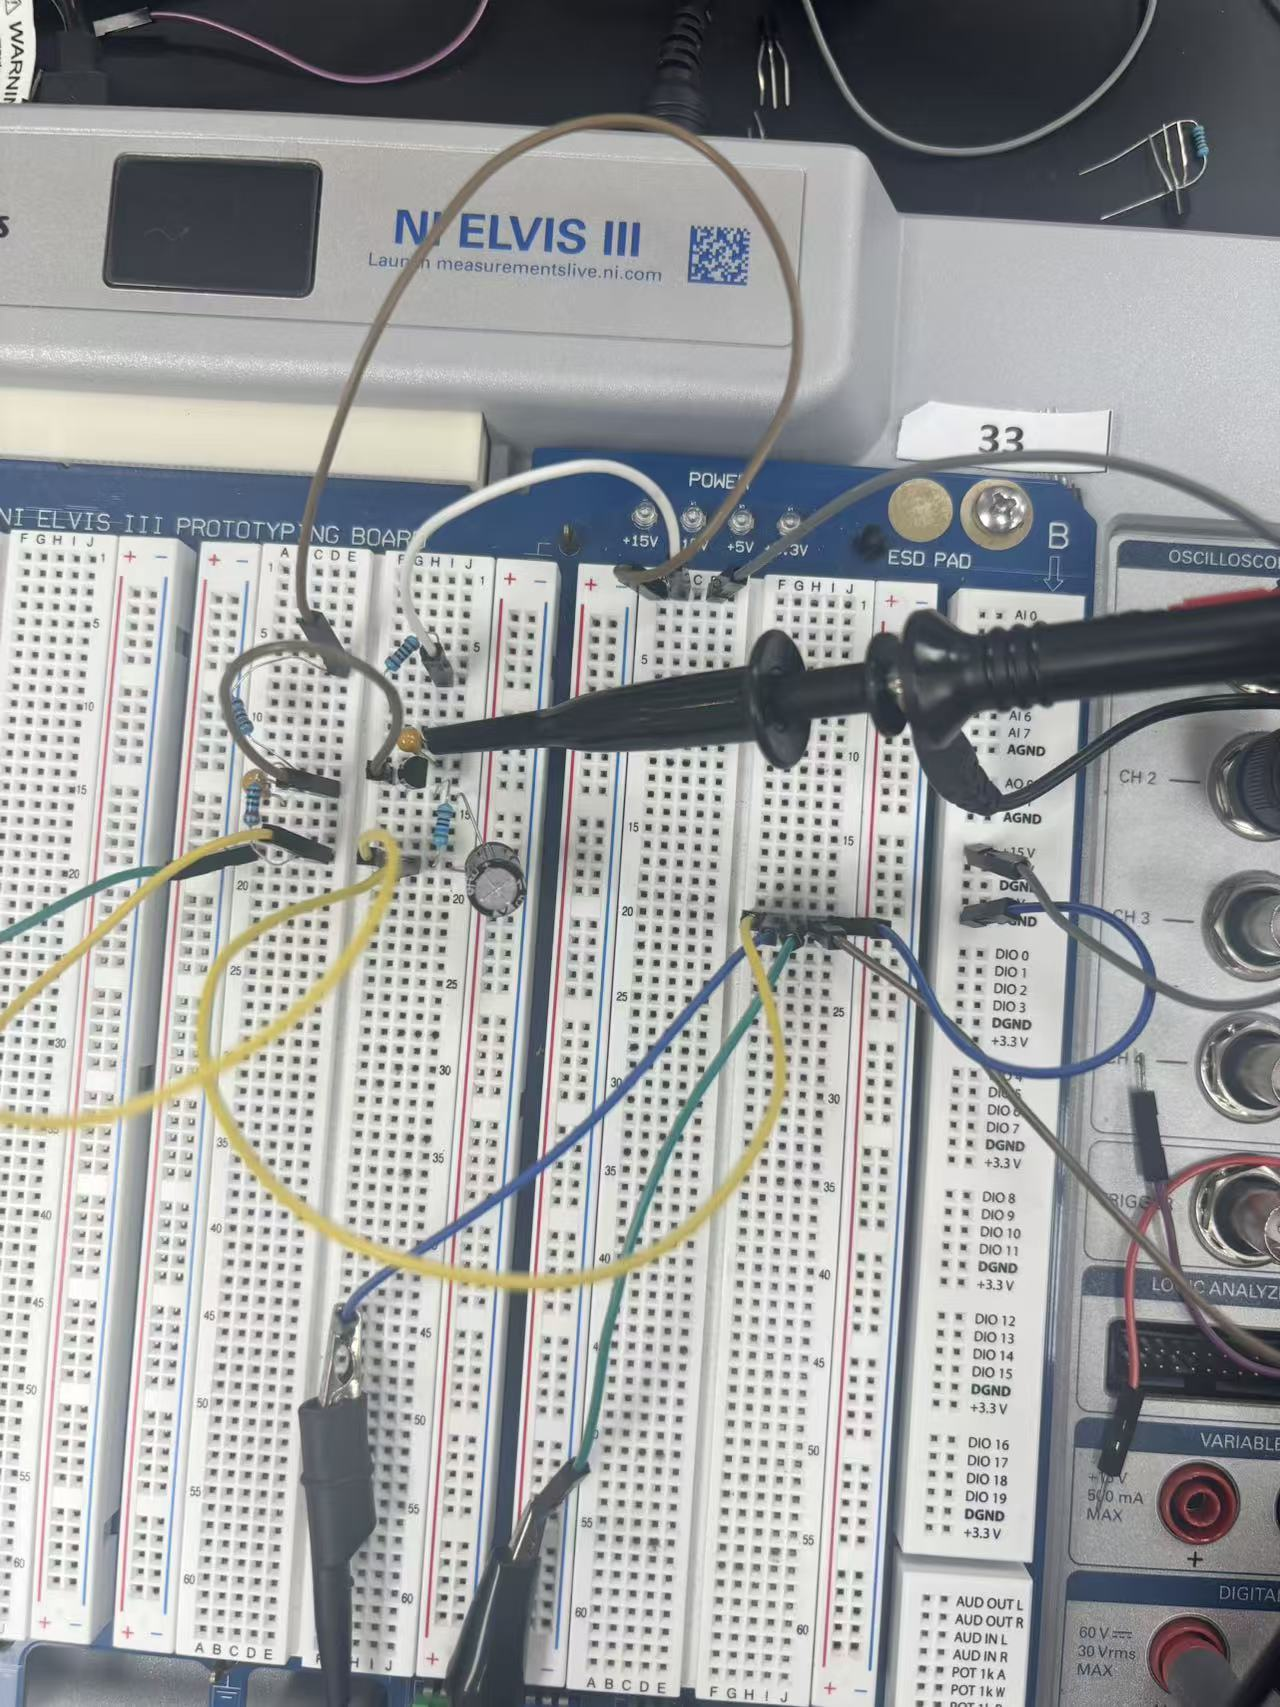
\includegraphics[width=0.50\textwidth]{Section3_Common_Emitter_Amplifier.jpg}

图：Section 3 共射放大器实际搭建
\end{center}

\subsection{Section 4: Emitter Follower Amplifier}
本部分采用仿真方法验证射极跟随器电路的特性。使用NI ELVIS III配套的仿真工具或第三方仿真软件（如SPICE）搭建射极跟随器电路模型。设置与实验脚本一致的元器件参数和工作条件，模拟输入阶跃或正弦信号，观察输出波形和频率特性。仿真结果包括输出电压与输入的关系（应接近1倍增益减去基极-发射极压降约0.6 V）、输入/输出阻抗等。

\begin{center}
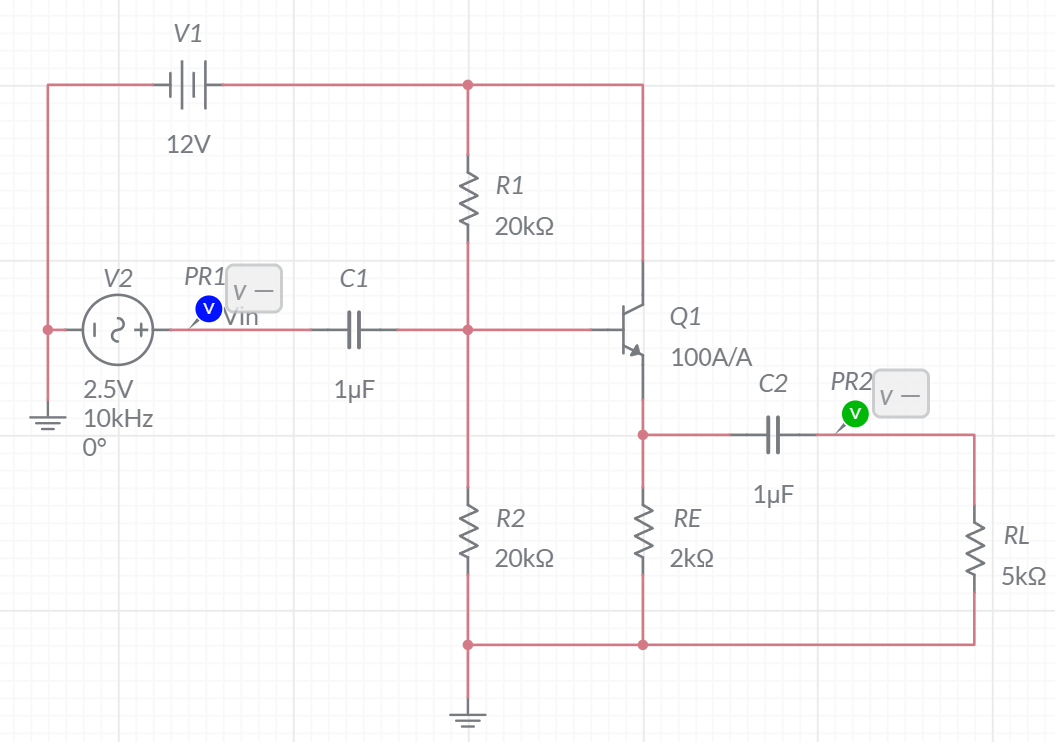
\includegraphics[width=0.45\textwidth]{Section4_Emitter_Follower_Diagram.png}

图：Section 4.1 射极跟随器电路原理图
\end{center}

\begin{center}
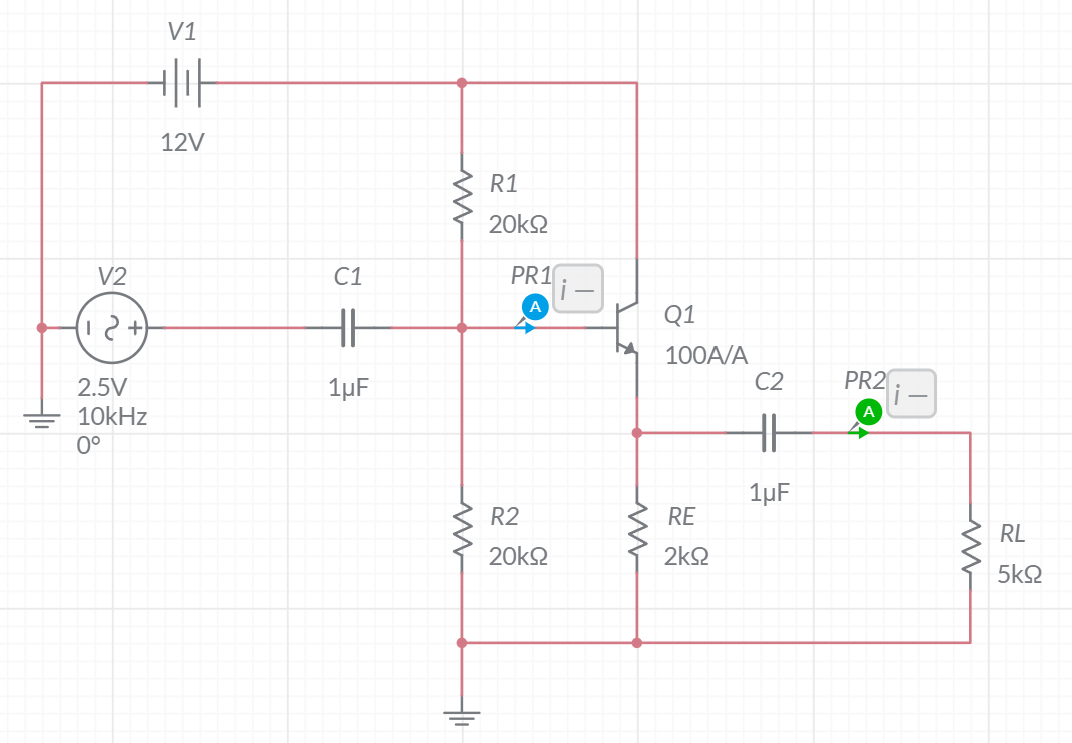
\includegraphics[width=0.45\textwidth]{Section4_Emitter_Follower_Circuit.png}

图：Section 4.2 射极跟随器电路图
\end{center}

\subsection{Section 5: Comprehensive Design Task}
本部分要求根据给定的设计规格（如输出电压、功率、纹波系数等）设计并搭建一个完整电路。该电路通常包含整流、稳压、可能的放大或其他功能模块。实验过程包括：（1）根据规格计算各级元器件参数；（2）在原型板上搭建电路；（3）使用NI ELVIS III的电源和DMM进行DC工作点测量；（4）在不同负载条件下测量输出特性；（5）记录电路工作状态的照片。

\begin{center}
\begin{minipage}{0.45\textwidth}
\centering
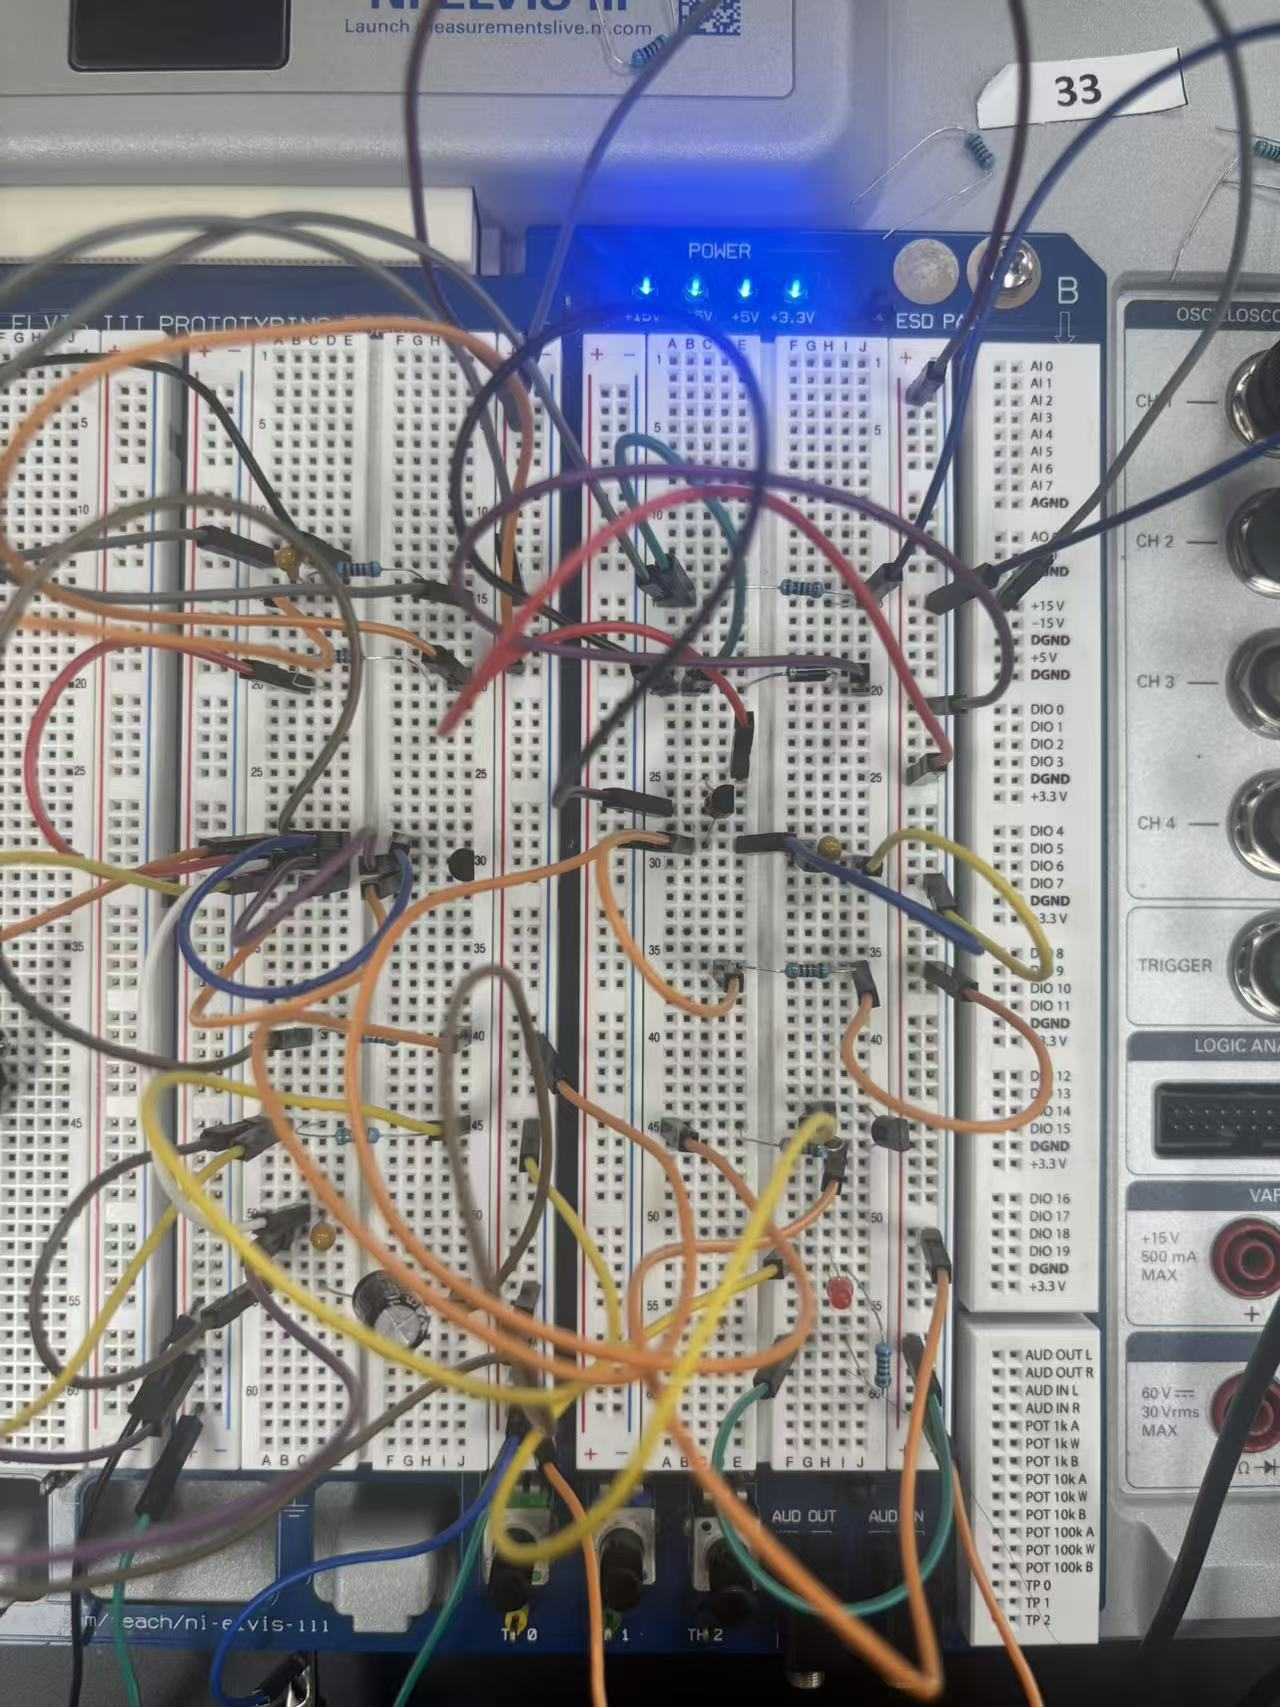
\includegraphics[width=\textwidth]{Section5_Design_Task_Off.jpg}

图：Section 5 设计任务电路（不工作状态）
\end{minipage}
\hfill
\begin{minipage}{0.45\textwidth}
\centering
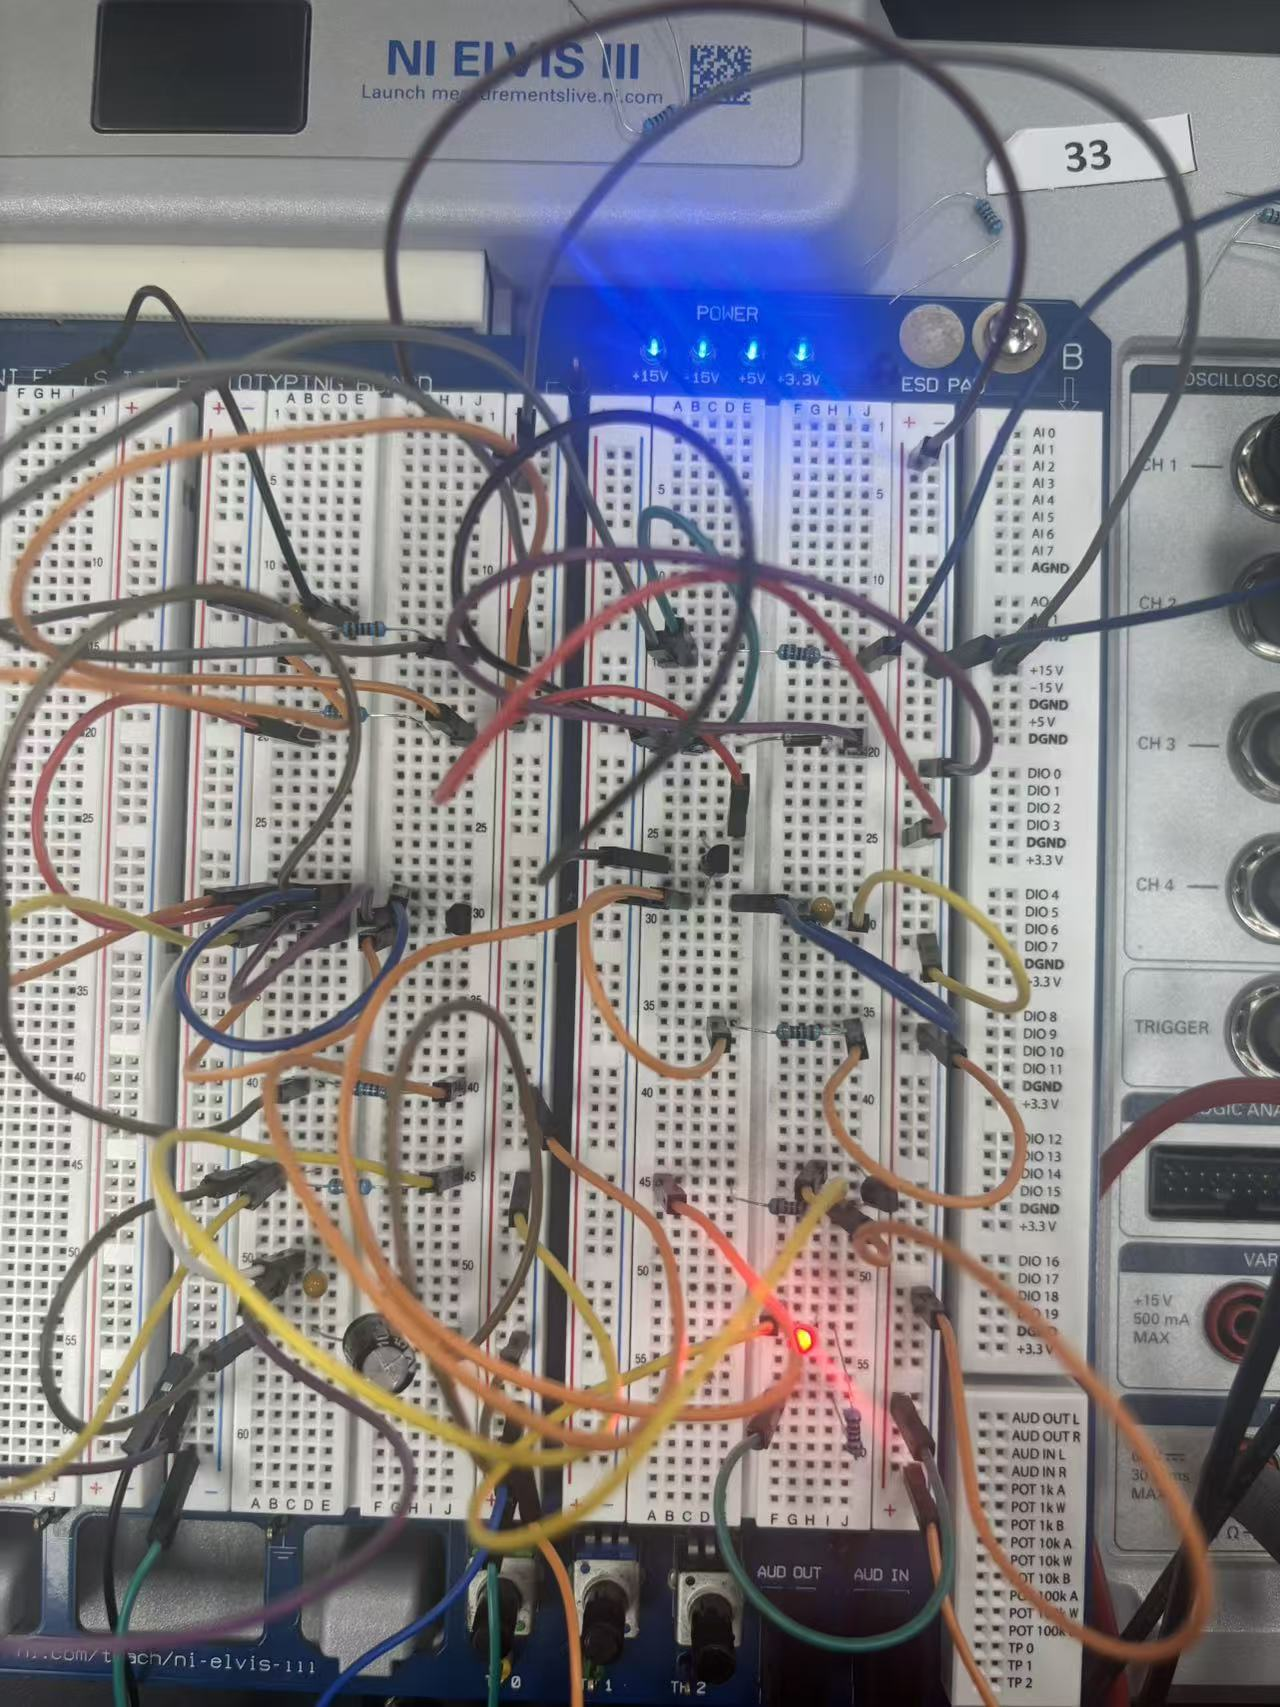
\includegraphics[width=\textwidth]{Section5_Design_Task_On.jpg}

图：Section 5 设计任务电路（工作状态）
\end{minipage}
\end{center}

\end{document}